\documentclass[xcolor=dvipsnames]{beamer}
%\usetheme{Pittsburgh}
\usepackage{pgfpages}
\usepackage{graphicx}
\usepackage{colortbl}
\usepackage{tikz}
\usepackage{pgfplots}
\usepackage{booktabs}
\usepackage[abs]{overpic}
\usepackage[scientific-notation=true]{siunitx}
\usetikzlibrary{decorations.pathreplacing}
\usetheme{MarburG}
\usecolortheme{whale}
\usepackage[ngerman]{babel}
\usepackage[utf8]{inputenc}
\newcommand{\pro}{\item[\boldmath${\color{green}+}$ ]}
\newcommand{\con}{\item[\boldmath$ {\color{red}-}$ ]}
\newcommand{\neutral}{\item[\boldmath$ {\color{black}\bullet}$ ]}

\usetikzlibrary{shapes.misc}
\usetikzlibrary{calc}
\tikzset{cross/.style={cross out, draw=red, minimum size=2*(#1-\pgflinewidth), inner sep=0pt, outer sep=0pt},
%default radius will be 1pt. 
cross/.default={1mm}}

\let\oldfootnotesize\footnotesize
\renewcommand*{\footnotesize}{\oldfootnotesize\tiny}

\newcommand{\tikzmark}[1]{\tikz[overlay,remember picture] \node (#1) {};}
\newcommand{\DrawBox}[1][]{%
    \tikz[overlay,remember picture]{
    \draw[red,#1]
      ($(left)+(-0.84cm,0.9cm)$) rectangle
      ($(right)+(-0.22cm,-0.2cm)$);}
}

\setbeameroption{hide notes} % Only slide
%\setbeameroption{show only notes} % Only notes
%\setbeameroption{show notes}
%\setbeameroption{show notes on second screen=left} % Both

\title{Lasttests von Webseiten mit JMeter}
\subtitle{Seminararbeit SS 2018}
\titlegraphic {
\includegraphics[width=2cm]{bilder/hskalogo_only}}
\author{Daniel Schäfer}
\date{\today}

%----------------------------------------------------------------------
\begin{document}

%titelseite------------
\begin{frame}
\titlepage
\end{frame}
%----------------------

%inhaltsverzeichnis----
\begin{frame}
\frametitle{Agenda}
		\tableofcontents
\end{frame}
%----------------------

%-------1--------------
\section{Einleitung}
\begin{frame}
\frametitle{Einleitung}
%\begin{overpic}[width=1\textwidth, grid, tics=10]{bilder/elephants}
\begin{center}
%\begin{overpic}[width=0.75\textwidth]{bilder/elephants}
%\put(10, 40){\footnote{\tiny Bildquelle: https://www.businessnewsdaily.com/6620-what-work-life-balance.html}}
%\end{overpic}
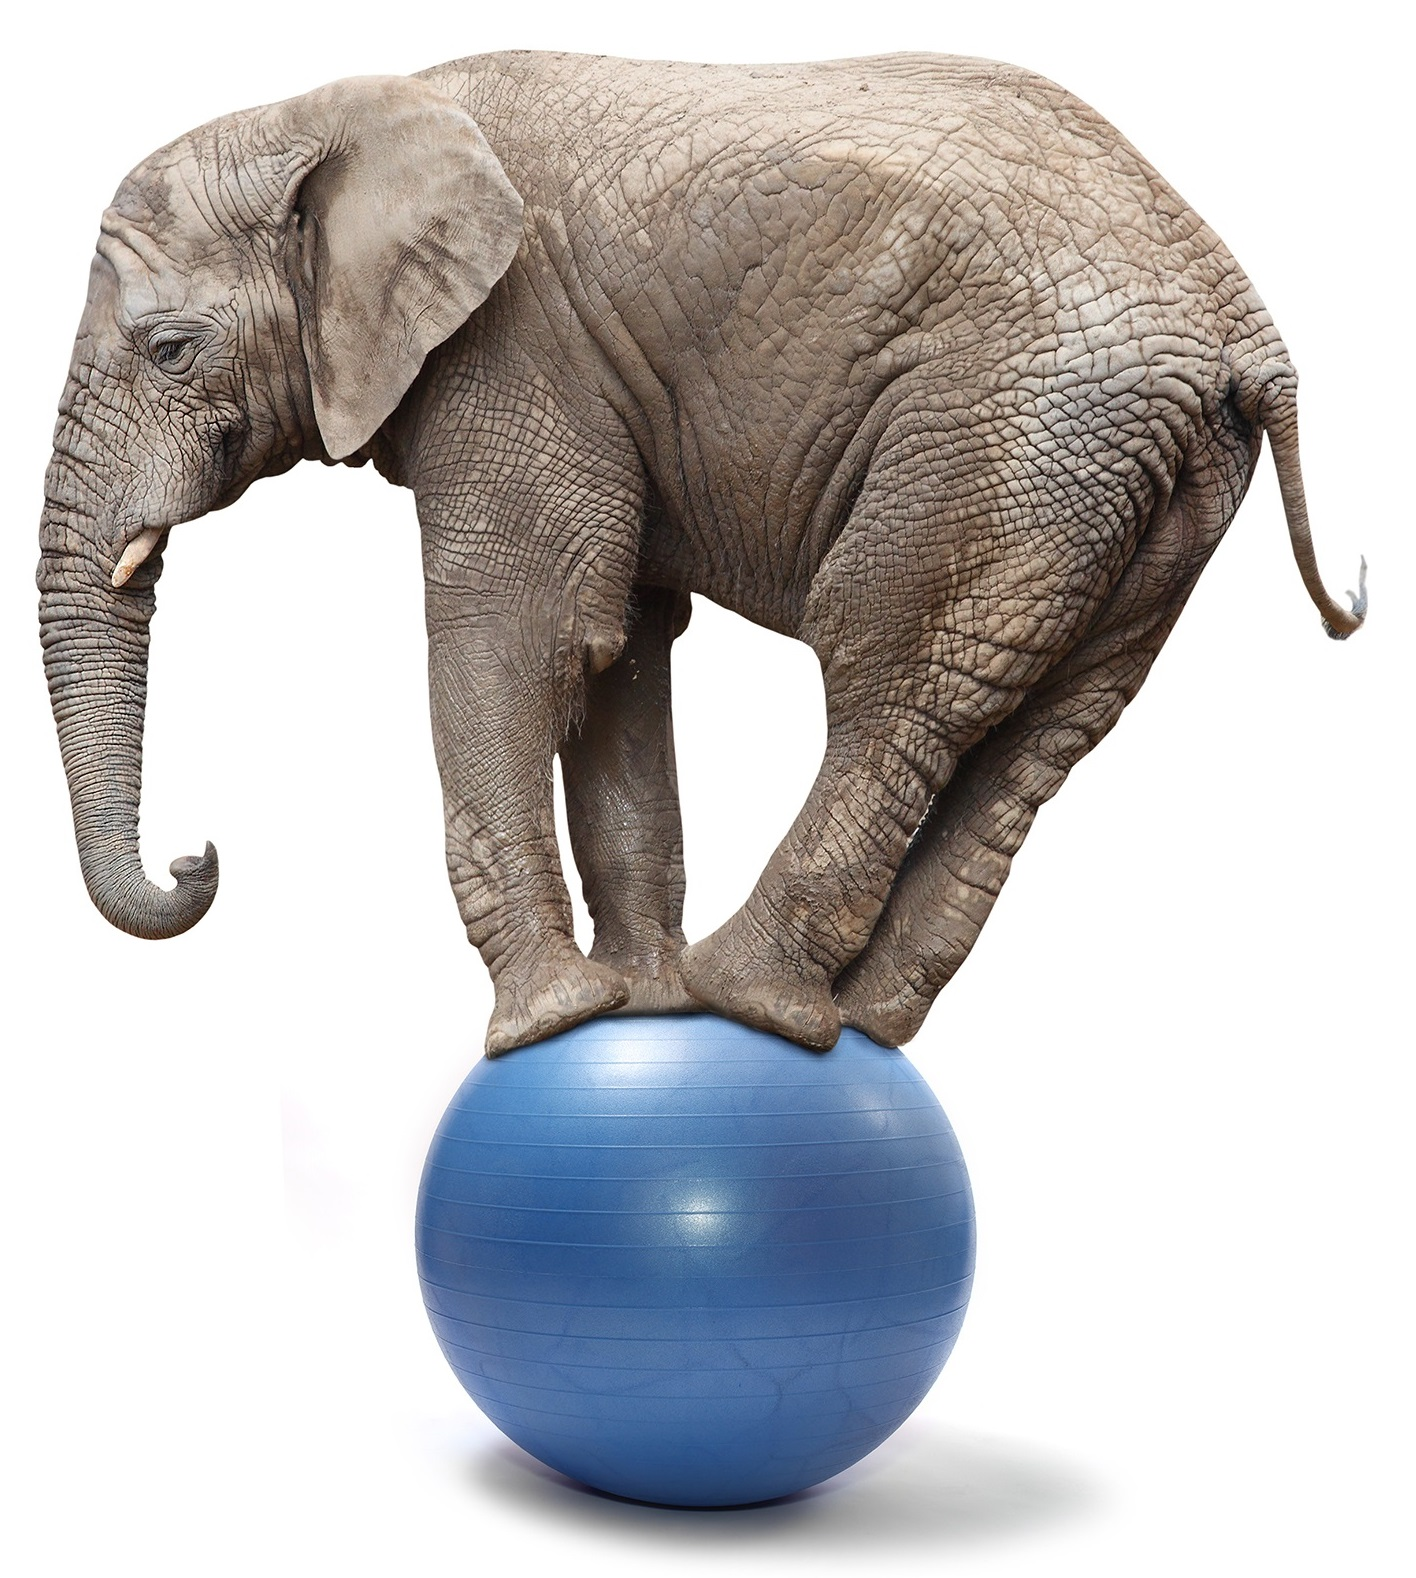
\includegraphics[width=0.7\textwidth]{bilder/elephants}
\footnote{\tiny https://www.businessnewsdaily.com/6620-what-work-life-balance.html}
\end{center}

\note{bild fand ich ganz passend. es stammt aus einem work life balance artikel aber trifft lasttest ganz gut. worum geht es? ich will kurz die motiviation ansprechen. wozu braucht man lasttests, danach basiswissen von lasttests vermitteln und was für anforderungen man benötigt.}
\end{frame}
%----------------------

%-------1.1------------
\subsection{Motivation}
\begin{frame}
\frametitle{Motivation}
\begin{center}
\includegraphics[angle=10, width=0.7\textwidth]{bilder/unerreichbar}
\end{center}
IWI-Intranet Seite geht am Anmeldetermin der Seminar/Projektarbeiten unter der Last in die Knie! 
\note{Bestes beispiel und dass dem herrn vogelsang immer wieder nachhängen wird ist die iwi seite, die unter der last in die knie ging. Weitere beispiele wie Neue Webseite oder Shop die viele Besucher erwartet, hat große Latenzzeiten oder
ist gar nicht mehr erreichbar (Worst Case) Greg Linden - Amazon hat ermittelt, dass sie pro 100ms verzögerung 1\% weniger verkaufserlöse haben. Daraus folgt Zeit = Geld / schneller = besser}
\end{frame}
%----------------------

%-------1.2.1----------
\subsection{Grundlagen Lasttests}
\begin{frame}
\frametitle{Grundlagen Lasttests}
\note{bei einem lasttest, wird wie der name es vermuten lasst hohe last auf einem system erzeugt und das verhalten untersucht. lasttests haben folgende ziele 1 2 3
lasttests sind oft die letzten schritte der entwicklung bevor die software eingeführt wird, was dazu verleitet diese so schnell wie möglich hinter sich zu bringen. man sollte sich dennoch genügend zeit für sie nehmen um am ende nicht noch eine böse überraschung zu erleben}
\textbf{Was sind Lasttests?}\newline
Bei einem Lasttest wird hohe Last auf einem System erzeugt und dessen Verhalten untersucht. \newline

\textbf{Wozu Lasttests?}
\begin{itemize}
		\item Erfüllung nicht funktionaler Anforderungen wie Antwortzeiten / Mengenbewältigung
		\item Dimensionierung von Hardwareresourcen  	
		\item Aufdeckung nicht gefundener Fehler (Nebenläufigkeit und blockierende Prozesse)
		\item Allgemein $\rightarrow$ Stabilität der Anwendung prüfen
	\end{itemize}
\end{frame}
%----------------------

%-------1.2.2----------

\begin{frame}
\frametitle{Grundlagen Lasttests}

\textbf{Manuelles Testen}
\begin{itemize}
\item "`echte"' Personen bedienen die Anwendung
\item Zeit- und resourcenintensiv \newline
\note{Man benötigt einige Benutzer, in kleineren Firmen oft die Entwickler selbst, die in dem Zeitraum nicht zur Verfügung stehen. man verwechselt häufig Lasttests mit UAT. user akzeptanztests sollten schon gemacht werden. allerdings mehr auf funktionalität bezogen und weniger auf die Last}
\end{itemize}

\textbf{Automatisiertes Testen}
\begin{itemize}
\item Tools wie JMeter, Gatling oder The Grinder
\item Simulation von vielen Benutzern (Threads)
\note{achtung man sollte parametrisierte werte wie passwörter/benutzernamen (base64) oder eventuelle captchas (einheitlich) im vorfeld beachten. } 
\end{itemize}
\end{frame}

%-------1.3------------
\subsection{Anforderungen an Lasttests}
\begin{frame}
\frametitle{Anforderungen an Lasttests}
\note{Ein lasttest sollte folgende fälle abdecken können: verschiedene lastvariationen, z.b. viele gleichzeitige anfragen über einen konstanten zeitraum, ab einer bestimmten tageszeit sehr viele zugriffe - spitzenzeiten, die antwortnachrichten sowie zeiten sowie der datendurchsatz sollte einsehbar sprich loggbar sein, die verteilung der tests auf mehrere server oder cloud dienste sollte machbar sein}
\begin{itemize}
\item Lastvarianten (Gleichzeitig Zugriffe, Spitzenzeiten)
\item Antwortzeiten und Datendurchsatz
\item Auf welcher Infrastruktur soll der Test laufen
\end{itemize}
\end{frame}
%----------------------

%-------2--------------
\section{Apache JMeter}
\begin{frame}
\frametitle{Apache JMeter}
\begin{center}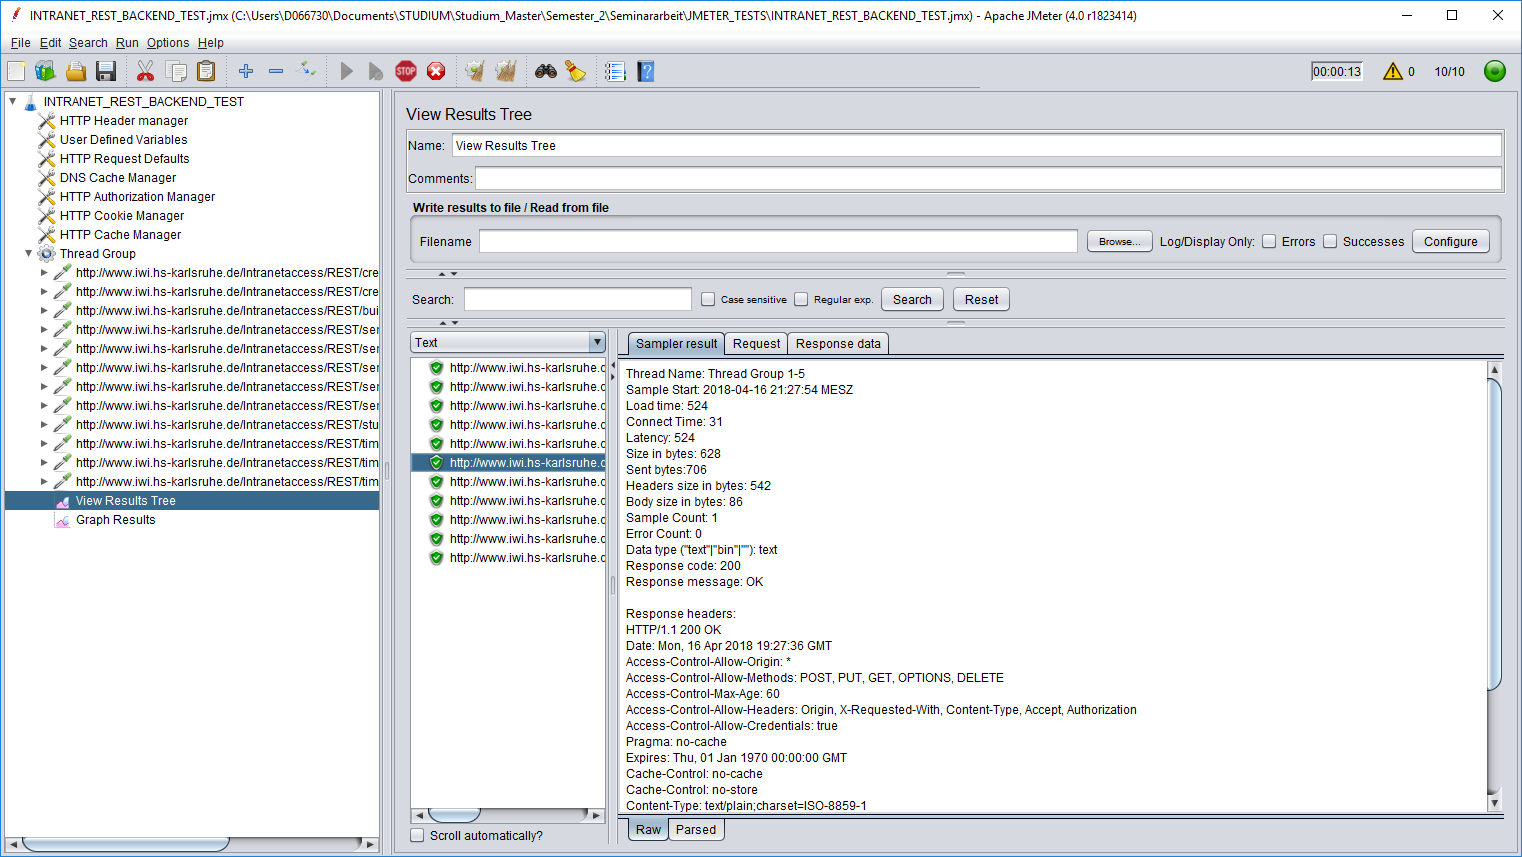
\includegraphics[width=1\textwidth]{bilder/jmeter_1}
\end{center}
\note{All dies bietet das open source Lasttestprogramm JMeter von Apache. version 1.0 wurde von Stefano Mazzocchi im jahr 1999 entwickelt um ursprüunglich die performance von Apache Tomcat zu testen. Hat sich daraufhin stetig weiterentwickelt und ist heute der de facto standard bei großkonzernen wie sap und 1und1 wo es regelmäßig im einsatz ist und den resourcenbedarf von anwendungen ermittelt. auf die hier abgebildete gui wird später genauer eingegangen }
\end{frame}
%----------------------


%-------2.1------------
\subsection{JMeter Übersicht}
\begin{frame}
\frametitle{JMeter Übersicht}

\begin{itemize}
\item Open Source / platformunabhängig (Java-Anwendung)
\item JMeter erzeugt Anfragen und somit Last auf Servern
\item Kann sehr viele Protokolle wie
\begin{itemize}
	\item HTTP (SOAP/REST)
	\item JDBC 
	\item FTP
	\item Beanshell (Java), JUnit
	\end{itemize}
\item GUI + Non-GUI-Modus
\note{gui um aufzeichnung zu erstellen und eventuell einfache tests zu machen. non gui in der cloud, performanter. man kann automatisiert ablaufen lassen}
\item Simulation von Benutzern (Threads)
\item Master-Slave-fähig für Cloud-Anwendungen
\item Umfangreiche Analyse-Funktionen
\end{itemize}
\end{frame}
%----------------------

%------2.2.1-----------
\subsection{Funktionsweise von JMeter}
\begin{frame}
\frametitle{Funktionsweise von JMeter}
\begin{enumerate}
\item Erstellung eines Testskripts durch Aufzeichnen von Browserinteraktionen
\item Parametrisierung z.b. durch Anzahl Benutzer, Benutzernamen, Passwörter, Servernamen, Ports
\item Lasttest ausführen 
\item Visualisierung und Analyse der Ergebnisse 
\note{Analyse dann durch Reports}
\end{enumerate}
\end{frame}
%----------------------

%------2.2-------------
\subsection{Die JMeter GUI}
\begin{frame}
\frametitle{Die JMeter GUI}
\note{sobald man jmeter heruntergeladen und entpackt hat, kann man es entweder via kommandozeile oder ausführen der jmeter exe aus dem bin verzeichnis starten. kommandozeile hat den vorteil dass man mehrere kommandos mitgeben kann, wie etwa ein html dashboard auf das ich noch später zurückkomme. auch ist der resourcenverbrauch deutlich geringer als mit der gui}
\begin{center}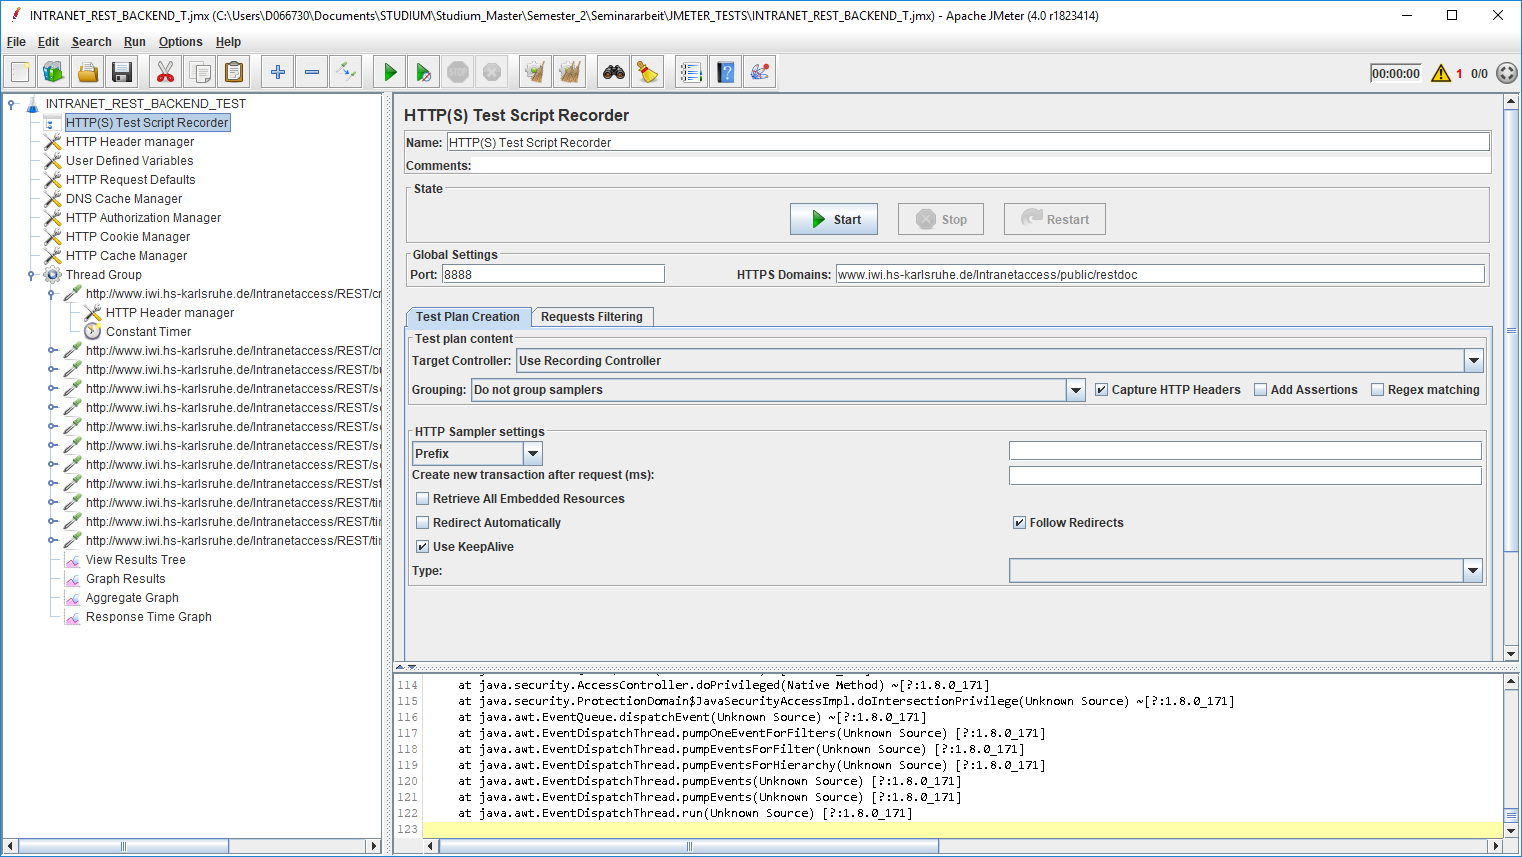
\includegraphics[width=1\textwidth]{bilder/jmeter_gui}
\end{center}
\end{frame}
%----------------------

%------2.3-------------
\subsection{JMeter Elemente}
\begin{frame}
\frametitle{JMeter Elemente}
\begin{tikzpicture}
\draw[shade, top color=blue!40!white] (0,8) rectangle (9.8, 0) node at (0.8, 7.6) {\small Testplan};
\end{tikzpicture}
\end{frame}
%----------------------

%------thread-gruppe-------------
\begin{frame}
\frametitle{JMeter Elemente}
\begin{tikzpicture}
\draw (0,8) rectangle (9.8, 0) node at (0.8, 7.6) {\small Testplan};
\draw[shade, top color=blue!40!white] (0.3,7) rectangle (9.5, 1.6) node at (1.6, 6.6) {\small Thread-Gruppe};
\end{tikzpicture}
\end{frame}
%----------------------

%------sampler-------------
\begin{frame}
\frametitle{JMeter Elemente}
\begin{tikzpicture}
\draw (0,8) rectangle (9.8, 0) node at (0.8, 7.6) {\small Testplan};
\draw (0.3,7) rectangle (9.5, 1.6) node at (1.6, 6.6) {\small Thread-Gruppe};
\draw[shade, top color=blue!40!white] (0.6 , 6) rectangle (9.2, 4) node at (1.4, 5.6) {\small Sampler};
\end{tikzpicture}
\end{frame}
%----------------------

%------controller-------------
\begin{frame}
\frametitle{JMeter Elemente}
\begin{tikzpicture}
\draw (0,8) rectangle (9.8, 0) node at (0.8, 7.6) {\small Testplan};
\draw (0.3,7) rectangle (9.5, 1.6) node at (1.6, 6.6) {\small Thread-Gruppe};
\draw (0.6 , 6) rectangle (9.2, 4) node at (1.4, 5.6) {\small Sampler};
\draw[shade, top color=blue!40!white] (5.7, 2.8) rectangle (7.8, 2) node at (6.6, 2.4) {\small Controller};
\end{tikzpicture}
\end{frame}
%----------------------


%------config-elemente-------------
\begin{frame}
\frametitle{JMeter Elemente}
\begin{tikzpicture}
\draw (0,8) rectangle (9.8, 0) node at (0.8, 7.6) {\small Testplan};
\draw (0.3,7) rectangle (9.5, 1.6) node at (1.6, 6.6) {\small Thread-Gruppe};
\draw (0.6 , 6) rectangle (9.2, 4) node at (1.4, 5.6) {\small Sampler};

\draw[shade, top color=blue!40!white] (0.9, 5.2) rectangle (3.6, 4.4) node at (2.2, 4.8) {\small Config-Elemente};

\draw[shade, top color=blue!40!white] (0.6, 2.8) rectangle (3.3, 2) node at (1.9, 2.4) {\small Config-Elemente};
\draw (5.7, 2.8) rectangle (7.8, 2) node at (6.6, 2.4) {\small Controller};

\draw[shade, top color=blue!40!white] (0.3, 1.1) rectangle (3.0, 0.3) node at (1.6, 0.7) {\small Config-Elemente};
\end{tikzpicture}
\end{frame}
%----------------------

%------listener-------------
\begin{frame}
\frametitle{JMeter Elemente}
\begin{tikzpicture}
\draw (0,8) rectangle (9.8, 0) node at (0.8, 7.6) {\small Testplan};
\draw (0.3,7) rectangle (9.5, 1.6) node at (1.6, 6.6) {\small Thread-Gruppe};
\draw (0.6 , 6) rectangle (9.2, 4) node at (1.4, 5.6) {\small Sampler};

\draw (0.9, 5.2) rectangle (3.6, 4.4) node at (2.2, 4.8) {\small Config-Elemente};
\draw[shade, top color=blue!40!white] (4.1, 5.2) rectangle (5.7, 4.4) node at (4.9, 4.8) {\small Listener};

\draw (0.6, 2.8) rectangle (3.3, 2) node at (1.9, 2.4) {\small Config-Elemente};
\draw[shade, top color=blue!40!white] (3.7, 2.8) rectangle (5.3, 2) node at (4.5, 2.4) {\small Listener};
\draw (5.7, 2.8) rectangle (7.8, 2) node at (6.6, 2.4) {\small Controller};

\draw (0.3, 1.1) rectangle (3.0, 0.3) node at (1.6, 0.7) {\small Config-Elemente};
\draw[shade, top color=blue!40!white] (3.4, 1.1) rectangle (5.0, 0.3) node at (4.2, 0.7) {\small Listener};
\end{tikzpicture}
\end{frame}
%----------------------

%-------2--------------
\section{Live Demos}
\begin{frame}
\frametitle{Live Demos}
\begin{itemize}
	\item Test von Threads im GUI Modus mit Graph 
	\item HTML-Dashboard erzeugen und analysieren
\end{itemize}
\end{frame}
%----------------------

 

\section{Fazit}	
\begin{frame}
	\frametitle{Fazit}
	\begin{itemize}
		\pro Platformunabhängig
		\pro Open-Source-Software
		\pro Testerstellung in GUI
		\pro Testlauf in GUI/Kommandozeile
		\pro Ergebnisse in HTML-Dashboard
		
		\con Swing Oberfläche
		\con Testpläne in XML-Format
		\con GUI resourcenhungrig
		
		\neutral Manuelle Zusammenstellung der REST-Endpunkte
		\neutral Keine Captcha-Erkennung
		
		\note{JMX Format ist eine XML Datei. Daher unhandlich ohne GUI werte zu ändern.
		
		jmeter ist ein super tool um die lasttests an webseiten auszuführen. es ist kostenlos hat viele tutorials und how-tos auf der offiziellen seite von apache. durch eine flache lernkurve bleibt man stehts motiviert sich weiter mit dem thema zu beschäftigen.

Die visualisierung der ergebnisse durch das html dashboard sind natürlich super.
		
gibt alternativen zu jmeter wie z.b. gatling oder selenium oder the grinder. wer lust hat kann sich gerne damit befassen. oder als nächste seminararbeit}
	\end{itemize}
\end{frame}

\subsection{Abschließende Worte}
%\subsection{Ausblick}
\begin{frame}
\frametitle{Abschließende Worte}
Die Funktionalität einer Anwendungen steht immer an erster Stelle. Erst wenn alle Anforderungen des Kunden erfüllt sind und noch Zeit/Budget vorhanden ist wird optimiert! 
\end{frame}

\begin{frame}
\begin{center}
\includegraphics[width=0.8\textwidth]{bilder/apache_logo}
\footnote{\tiny https://jmeter.apache.org/}
\end{center}
\end{frame}

\end{document}